This chapter will build our approach to user modeling.
We will first explain why a new approach is needed,
and outline a few hypotheses that will test our reasoning.
We shall then develop \emph{stacked user modeling},
a novel approach to adaptive user model aggregation.
The last parts of this chapter shows how this new approach
can perform prediction aggregation in a recommendation scenario,
and rank aggregation in an information retrieval scenario.

\section{The Latent Subjectivity Problem}
\label{sec:reasoning}

As we saw in Chapter \ref{chap:theory}, 
there are lots of ways of predicting the
relevance of an item to a user. 
In fact, judging by the number of different approaches,
the only limiting factor seems to be the different 
patterns researchers discover in available data.
As described in Section \ref{sec:aggregate},
modern approaches to recommender systems try to combine many of these methods.
Aggregate modeling is a common way of combining different, complimenting
methods into one prediction system.
By leveraging so called \emph{disjoint patterns}
in the data, several less than optimal predictors
can be combined, so that the combination outperforms each part.
Moderns search engines work much in the same way,
combining multiple ranking signals into a final results list
(see Section \ref{subsec:signals}).

Why then, when we have all these valid approaches, would we need yet another technique?
We posit that both simple predictors and aggregation methods have a fundamental problem.
There exists an underlying, misplaced subjectivity to relevance prediction that is seldom discussed.

When a method is developed or selected for use in a prediction system,
a concious descision of which approach to use is made.
Before any user modeling is performed, the researcher or developer selects
one or more methods that is thought to best model every user and item in the system.
Should it not be up to each user to decide which method best describes their preferences?
And, considering the vast scope of items we can come by, will the selected
methods perform similarly for every item?

Consider the following examples of relevance judgement:

\begin{itemize}
  \item PageRank \citep{Bender2005} assumes that the relevance of a web page is 
  represented by its authority, as computed from inbound links from other sites.
  \item Some systems considers a user's social connections to be important
  in ranking search results, when performing personalized search (e.g. \cite{Carmel2009}).
  \item When recommending movies, one predictor may be based on the ratings
  of users with similar profile details. Another predictor might be 
  dependent on some feature, e.g. production year of well liked movies.
  \item Recommendations based on the Pearson Coefficient \cite[p11]{Segaran2007}
  assumes that the statistical correlation between user ratings is a good
  mesure for user similarity.
\end{itemize}

Are these metrics subjective? 
While the methods themselves may perform well, their selection
reflects how whoever created the system assumes how each user
can and \emph{should} be modeled. This underlying subjectivity is not desirable.
We call this the \emph{latent subjectivity problem}.

Examples of this problem are not hard to come by.
For instance, while one user might appreciate a social
influence in their search results, another user might not.
While one user might find frequency of communication maps well to relevance,
another might not. 
One user might feel the similarity of movie titles are a good predictor,
while another might be more influenced by production year.
The exact differences are not important --- what is important is that they exist.
The same goes for items: while one item might best be judged by its content,
another might be better described by previous ratings from other users.
One item's relevance may be closely tied to when it was created,
while other items may be timeless.

Another way of explaining the latent subjectivity problem is that 
\emph{user modeling methods are dependent on the subjective assumptions of their creators}.
In other words, a modeling method use some aspect of available data to make predictions,
and this aspect is chosen by whoever creates the system.
Aggregate modeling methods face the same problem of misplaced subjectivity: 
Aggregation is done on a generalized, global level,
where each user is expected to place the same importance on each modeling method.
While the aggregation is of course selected to minimize some error over a testing set,
the subjective nature remains: The compiled aggregation is a generalization,
treating all users the same --- hardly a goal of user modeling.

We propose a method where these descisions are left to each user and item,
providing an extra level of abstraction and personalization.
This leaves the subjective nature of selecting ways to model users and items where it should be:
In the hands of each individual user, and dependent on each specific item.
If each method is \emph{only used} based on how well it performs for each element,
any possibly applicable recommender system suddenly becomes a worthy addition to the system.
Imagine creating a recommendation system, and consider the following two questions:

\begin{enumerate*}
  \item What combination of which methods will accurately predict unknown scores?
  \item Which methods could possibly help predict a score for a user or an item?
\end{enumerate*}

The first question is what has to be considered in traditional modeling aggregation:
First a set of applicable methods leveraging disjoint patterns must be selected. 
Then, an optimal and generalized combination of these must be found,
most often through minimizing the average error across all users.

The second question is quite different. 
Instead of looking for an optimal set of methods and an optimal combination,
we look for the set of \emph{any applicable methods} that \emph{some users} might find helpful,
or that might work for \emph{some items}.
We believe this is a much simpler problem: 
instead of trying to generalize individuality,
it should be embraced, by allowing users to implicitly and automatically select which methods they prefer,
from a large set of possible predictors.

Just as each user is different, each item may have their own characteristics.
Needless to say, items are often quite different from another,
along a myriad of dimensions. Consider the World Wide Web:
If each webpage is an item, the number of metrics we can use to judge
the relevance of an item is immense.
If items are indeed as different as the users themselves, it stands to reason that the same 
modeling method will not perform as well for every item.

As before, an approach where we only need to consider the second question is desireable.
Regardless, both traditional, single-approach modeling methods, and modern aggregation approaches
often treat every item the same. No matter its intrinsic qualities, an item will be judged
by the same methods as every other item. 

This chapter will develop a way to aggregate a host of modeling methods on a per-user and per-item basis.
By adapting the aggregation to the current item and user, we sidestep the latent subjectivity problem. 
The user is in control of which methods best fit their needs, and
each method's priority is influenced by how well it performs for the current item.
We will now express our goals as a three hypotheses.


\section{Three Hypotheses}
\label{sec:hypotheses}

To evaluate whether or not \emph{stacked user modeling}
can mitigate the latent subjectivity problem,
we need a set of hypotheses.
To solve the subjectivity problem we need our modeling method
to adaptively aggregate a set of predictions based on the current user and item.
In other words, by automatically adapting how a set of disjoint recommenders
are combined, based on each user and item, we should be able to achieve a
result that is better than each of the stand-alone recommenders.
This adaptive method should also outperform other, generalized aggregation approaches.

This paper will consider three hypotheses (H1-H3) 
to establish whether adaptive aggregation through stacked user modeling is a viable technique.
H1 and H2 will consider the approach in regard to prediction aggregation
in a recommendation scenario. H3 will consider using this approach for
rank aggregation in an information retrieval scenario.
Let us start with prediction aggregation:

{
  \itshape
  $\mathbf{H1}$: The accuracy of relevance predictions can be improved
  by blending multiple modeling methods on a per-user and per-item basis.
}

It stands to reason that if a recommender system is indeed impaired
by the subjective selection of modeling methods,
an adaptive combination of these methods should outperform each of the individual approaches.
Second:

{
  \itshape
  $\mathbf{H2}$: An adaptive aggregation method can outperform global and generalized 
  blending methods.
}

If our assumption that model aggregation inherits the subjective nature of its chosen parts,
an adaptive aggregation without such misplaced subjectivity should outperform a
generalized combination.
Third:

{
  \itshape
  $\mathbf{H3}$: The result set from an information retrieval query
  can be personalized by stacked user modeling, where the retrieval scores are considered 
  standard input signals.
}

As described in Section \ref{subsec:signals},
modern search engines combines multiple ranking functions called signals into a final results list.
Each signal, be it an IR score, a metric like PageRank, or the result of a user modeling method,
contributes to the final item ranking.
We shall use H3 to see whether or not stacked user modeling can be used for this type of rank aggregation,
where a set of recommender systems constitute a set of input signals.

By answering our three hypotheses, it should become clear whether or not our approach
is a valid method of predicting the relevance of an item to a user.
These hypothesess will be tested in the next chapter, but first, let us build
the model we shall test.


\section{User Meta Modeling}

So, how do we perform personalized method aggregation?
Let us first define a few terms.
We define \emph{Meta Modeling} (MM) as using one modeling method to adapt other modeling methods.
More specifically, \emph{User Meta Modeling} (UMM) means adapting user modeling methods with another user modeling method.
This leaves us with two distinct levels of user modeling methods: the \emph{methods level} and the \emph{aggregation level}.
Formally, a system for UMM can be described as a 6-tuple:

\begin{eqnarray*}
  \mathrm{UMM} &=& (Items, Users, Ratings, Framework, Methods, Aggregation)\\
               &=& (I,U,R,F,M,A).
\end{eqnarray*}

We have a set of $Items$ and a set of $Users$.
There is also a set of $Ratings$: each user $u \in U$ can \emph{rate} an item $i \in I$.
As before, we use the term "rating" loosely --- other applicable and equivalent terms include \emph{relevance}, \emph{utility},
\emph{connection strength} or \emph{ranking}. In other words, this is a measure of what a user thinks of an item
in the current domain language. However, since "rating" will match the case study we present later in this chapter,
that is what we shall use. 

The $Framework$ variable specifies how this data is represented.
The two canonical ways of representing users, items and ratings are graphs and matrices (see Section \ref{sec:recommender}).
We shall use a matrix, where the first dimension corresponds to users, the second to items, and each populated cell is an explicit rating:

\begin{equation*}
 R_{u,i} =
 \begin{pmatrix}
  r_{1,1} & r_{1,2} & \cdots & r_{1,i} \\
  r_{2,1} & r_{2,2} & \cdots & r_{2,i} \\
  \vdots  & \vdots  & \ddots & \vdots  \\
  r_{u,1} & r_{u,2} & \cdots & r_{u,i}
 \end{pmatrix}
\end{equation*}

As we are dealing with multiple approaches to user modeling, we have a set of $Methods$ that each create their own
user models. 
This corresponds to the \emph{methods layer}.
Each model $m \in M$ are used to compute predictions, i.e. estimations of unknown ratings.
As demonstrated in Chapter \ref{chap:theory}, there are many different forms of user modeling,
that each consider differents aspects of the available data: the users, items and ratings, as well as 
other sources such as intra-user connections in social networks or intra-item connections in information retrieval systems.
Examples include Slope One, SVD and Nearest Neighbor weighted predictions
(see Section \ref{subsec:recommender:examples}).
These methods predict unkown connections between users and items based on some pattern in the data,
for example user correlations or social connections.

The $Aggregation$ part of our 6-tuple refers to how the predictions from the different methods are blended
into one prediction. 
This corresponds to the \emph{aggregation level}.
To achieve the best possible compounded result, we wish to use methods that look at disjoint patterns, 
i.e. complementary predictive parts of the data (see Section \ref{sec:aggregate}).
As found by \citet[p6]{Bell2007} the accuracy of the combined predictor is more dependent on the 
ability of the various predictors to expose different aspects of the data, than on 
the individual accuracy of each predictor.
As described in Section \ref{sec:aggregate}, multiple prediction results are normally 
combined into a final singular result,
based on a generalized combination found by minimizing some error across all users.

Another way of describing (and implementing) the two modeling levels is through application
of the $\mathrm{map}$ and $\mathrm{reduce}$ functions of functional programming.
When performing \emph{prediction aggregation} (scores), this estimation can be expressed as

\begin{equation*}
  \hat{r}_{ui} = \mathrm{reduce}(u, \mathrm{map}(M,u,i)).
\end{equation*}

First, each modeling method is applied through the $\mathrm{map}$ function, with the current user and rating for which
a rating should be estimated. This produces a set of scalar prediction values. These values are then
combined through the $\mathrm{reduce}$ method, which takes the predictions and current user as input.
In our case, this is the personalized aggregation method. 
If we wish to do rank aggregation (i.e. sorted lists), the equation is a bit different:

\begin{equation*}
  \tau_{u,n} = \mathrm{reduce}(u, \mathrm{map}(M,u,n)).
\end{equation*}

Here, $\tau_{u}$ is the list of recommended items for user $u$ (following the notation in \citet[p3]{Dwork2001}).
Note that there is no input item in this formula as we wish to produce a ranking of the top $n$ recommended items.

Expressing ourselves in terms of $\mathrm{map}$ and $\mathrm{reduce}$ now is helpful, as this will later
guide our implementation of these operations in a proper MapReduce framework
for parallell computation (as explained in \citet[p75]{Manning2008}).
The $\mathrm{map}$ function may apply each modeling method in parallell, 
as these are independent computations.
The modified $\mathrm{reduce}$ function, which takes the resulting predictions $\mathrm{map}$ and the current
user as inputs, serve as our personalized aggregator.
Let us now describe how to make this function.


\subsection{Personalized Aggregation}

To perform UMM, we need the $Aggregation$ (or $\mathrm{reduce}$) method to be an actual user modeling method,
that adapts the blending with respect to each user.
Until now we have talked about both prediction aggregation (scores) and rank aggregation (sorted lists).
For now we shall stick to scalar predictions, but will return to rank aggregation in Section \ref{sec:methods:rank}.

The simplest generalized way of prediction aggregation is a simple avereage over all predictions made
by the different methods (e.g. \citet[p3]{Aslam2001}):

\begin{equation*}
  \hat{r}_{ui} = \frac{1}{N} \sum_{m \in M} p_m(u,i).
\end{equation*}

$\hat{r}_{ui}$ is the estimated rating from user $u$ to item $i$,
$N$ is the number of methods in $M$, and $p_m(u,i)$ is the predicted rating from method $m$.
However, in most cases we wish to weight each method differently (e.g. \cite{Claypool1999} ):

\begin{equation*}
  \hat{r}_{ui} = \sum_{m \in M} w_{m} \cdot p_m(u,i) 
  \quad \text{where} \quad 0 \leq w_{m} \leq 1, \quad \sum_{i \in M} (w_i) = 1.
\end{equation*}

Here, $w_m$ is the weight applied to modeling method $m$. These weights fall in the range $[0,1]$ and sum up to $1$.
As described in \ref{sec:aggregate}, these weights can be estimated using a host of machine learning methods.
The known rating data is separated into a training- and testing set, which is used to estimate optimal weights
by minimizing some error across the testing set 
(note that the training set is also split in some way into two sets to create the singular modeling methods).
However, as discussed in Section \ref{sec:reasoning},
this is still a generalized, averaged result across every user. 
The system assumes that the best average result is the best result for each individual user.

So, in order to leverage as many data patterns as possible and to remove the latent subjectivity,
we wish the weights to be user-specific. The simplest approach is to create secondary user models for aggregation.
Intuitively, a user-specific weight vector could fill the role of this user model:

\begin{equation*}
  \hat{r}_{ui} = \sum_{m \in M} w_{um} \cdot p_m(u,i),
  \quad \text{where} \quad 0 \leq w_{um} \leq 1, \quad \forall u \in U: \sum_{i \in M} (w_{ui}) = 1.
\end{equation*}

where $w_{um}$ is the user specific weight for method $m$. In other words, $w_{u}$ is the user model vector.
Each user then has a pesonal set of weights describing how much they prefer each modeling method.
These weights can be estimated much in the same way as generalized weights, 
with the same training and testing set, just on a per-user basis.

However, a personalized linear combination of modeling methods is not enough.
Because of the disjoint nature of the differing modeling methods, 
they essentially each find some reason that an item should receive a certain score.
Consider the different patterns recommender systems and information retrieval measures might leverage:

\begin{itemize*}
  \item Ratings from other users weighted by user similarity.
  \item The similarity of items through the use of an IR method.
  \item Clustering items and users through global effects, finding general trends.
  \item Ratings based on local averages, generosity and other individual features.
  \item Comparing user preference terms with items.
\end{itemize*}

While a linear combination of such disjoint patterns may achieve accurate scores,
a nonlinear combination should be able to discover less apparent user preferences.
For example, in any case where the agreement of two or more methods are more telling than their contribution
to a linear combination, a nonlinear combination can catch such features of the user's preferences.

Consider the task of sorting incoming emails based on user preferences: 
a user might consider a new mail important if the sender is a social connection
and the last communication from this person happened a long time ago. 
In this case, the agreement between two scoring methods is more important
than any other prediction.

Another case is when one method is especially important for some 
range of its possible predictions. For example, if one method deals with catching possible spam,
a confident capture from this method would probably be more important than 
what any of the other predictions.

In short, we want an aggregation method capable of capturing nonlinear preferences
when it comes to combining user modeling methods.
Let us express this as an equation:

\begin{equation*}
  \hat{r}_{ui} = f_{u}(M(u,i))
\end{equation*}

The user model is the nonlinear function $f_u$ that takes the results of each modeling method $M(u,i)$,
and combines them to one prediction.
In other words, to achieve a nonlinear personalized aggregation, we need to train one function per user,
that takes a set of scalar scores and produces one scalar output.
One way of doing this is using a simple neural network, as we shall now explain.

\subsection{Multilayer Perceptron}

An \emph{artificial neural network} (ANN) is a computational model in AI,
inspired by aspects of biological neural networks.
They are represented as graphs, consisting of a set of nodes (representing artificial neurons) and
edges (representing synapeses).
ANNs can be used as statistical data modeling tools, capable of learning complex
relationships between input and output data
(see \citet[p567]{Russell1995} or \citet[p163]{Floreano2008}).

A \emph{multilayer perceptron} (MP) is a simple 
feedforward artificial neural network,
that maps a set of scalar inputs to a set of outputs,
and is capable of distinguishing data that is not linearly separable
\cite[p578]{Russell1995}.
This fits our needs for a personalized aggregation function.
By training a separate MP for each user, based on known ratings from this user,
we can create individual nonlinear functions for mapping multiple 
predictions to one output.

An MP has multiple layers: an input layer, one or more hidden layers, and an output layer.
Each layer has a set of nodes.
Every node in every layer is connected to all nodes in the next layer
with weighted edges (see Figure \ref{fig:neural}).
During network activation, values propagate from the input layer, through intermediary nodes and edges,
to the output layer. 

The input layer nodes corresponds to each input we wish to process,
and their value is set to the current raw input values.
For example, if the inputs are recommender system methods,
each input node corresponds to the prediction from one method.
Nodes in the hidden and output layer use a nonlinear activation function 
to capture patterns in the input data.
Depending on the input layer values, nodes in the first hidden layer
are either activated or not, and propagates some value to the 
following layer. This continues until we reach the output layer,
where the node(s) produce some final output value(s).

\begin{figure}[t]
  \center
  \def\layersep{4cm}
  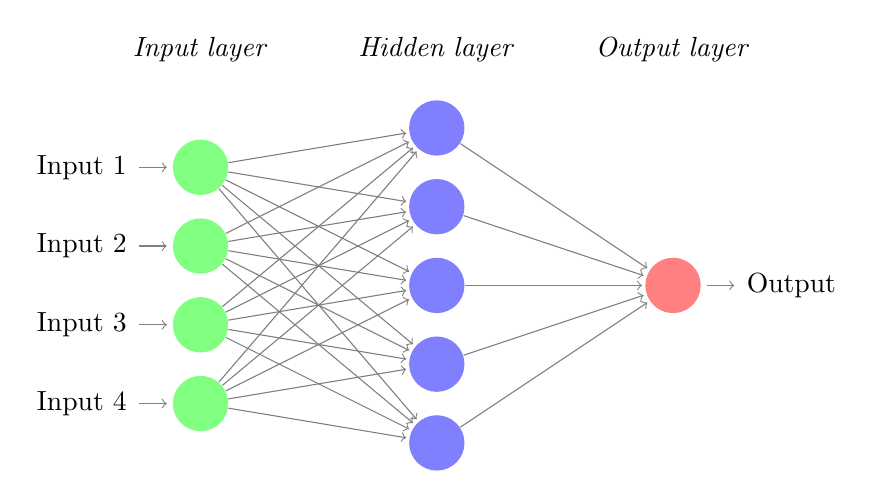
\begin{tikzpicture}[shorten >=1pt,->,draw=black!50, node distance=\layersep]

    \tikzstyle{every pin edge}=[<-,shorten <=2pt]
    \tikzstyle{neuron}=[circle,fill=black!25,minimum size=20pt,inner sep=0pt]
    \tikzstyle{input neuron}=[neuron, fill=green!50];
    \tikzstyle{output neuron}=[neuron, fill=red!50];
    \tikzstyle{hidden neuron}=[neuron, fill=blue!50];
    \tikzstyle{annot} = [text width=10em, text centered]

    % Draw the input layer nodes
    \foreach \name / \y in {1,...,4}
    % This is the same as writing \foreach \name / \y in {1/1,2/2,3/3,4/4}
        \node[input neuron, pin=left:Input \y] (I-\name) at (0,-\y) {};

    % Draw the hidden layer nodes
    \foreach \name / \y in {1,...,5}
        \path[yshift=0.5cm]
            node[hidden neuron] (H-\name) at (\layersep,-\y cm) {};

    % Draw the output layer node
    \node[output neuron,pin={[pin edge={->}]right:Output}, right of=H-3] (O) {};

    % Connect every node in the input layer with every node in the
    % hidden layer.
    \foreach \source in {1,...,4}
        \foreach \dest in {1,...,5}
            \path (I-\source) edge (H-\dest);

    % Connect every node in the hidden layer with the output layer
    \foreach \source in {1,...,5}
        \path (H-\source) edge (O);

    % Annotate the layers
    \node[annot,above of=H-1, node distance=1cm] (hl) {\emph{Hidden layer}};
    \node[annot,left of=hl] {\emph{Input layer}};
    \node[annot,right of=hl] {\emph{Output layer}};
  \end{tikzpicture}

  \vspace{1em}
  \caption[Multilayer Perceptron]{
  A multilayer perceptron with 4 input nodes, 1 hidden layer of 5 nodes
  and a single output node.
  Nodes in the hidden and output layers use a nonlinear activation function.}
  \label{fig:neural}
\end{figure}


A node's \emph{activation value} is its actual output value when the network is activated,
determined by an \emph{activation function}.
The use of hidden layers and nonlinear activation functions is what allows an MP
to separate nonlinear patterns. 
Every activation function relies on the weighted sum of the neuron's inputs $a_i$
\cite[p178]{Floreano2008}:

\begin{equation*}
  a_i = \sum_{j=1}^{N} w_{ij} x_j,
\end{equation*}

where $i$ and $j$ are nodes, $N$ is the number of input nodes to node $i$,
$w_{ij}$ is the weight of the connection between the two nodes,
and $x_{j}$ is the activation value of node $j$.
There are many possible activation functions,
each applicable to some domains and types of data.
Two common choices are the following two sigmoid functions
\cite[p179-180]{Floreano2008}:

\begin{equation*}
  \Phi(a_i) = tanh(a_i) \quad \text{and} \quad \Phi(a_i) = \frac{1}{1 + e^{-a_i}}.
\end{equation*}

The first function is the hyperbolic tangent which falls in the range $[-1,1]$,
while the second is an equivalent function in the range $[0,1]$.
Other possible activation functions include
gaussian distribution functions, ramp and step functions, and trapezoidal
functions.

The \emph{backpropagation algorithm} for supervised learning \cite[p578]{Russell1995}
is used to train an MP.
This iterative algorithm uses a set of training examples to adjust the weights in 
the network. Each training example is a set of input values with a corresponding correct output value.
Backpropagation works in two phases:

(1) The first phase begins by activating the network with an example from the training set,
which produces an actual output value based on the current network configuration.
The error between this actual output and the desired output from our example
is propagated back through the network, which generates deltas (differences)
between the actual neuron outputs and desired neuron outputs.

(2) The second phase adjusts the weights of the network edges based on the computed error deltas.
This output delta is multiplied with the input activation value to get the gradient of the weight,
signifying how much the weight is wrong and in which direction.
The weight is adjusted in the opposite direction of the gradient by subtracting some ratio
of the gradient from the weight. 
This ratio is called the \emph{learning rate},
and can be adjusted to change the speed and quality of learning in the network.

When the network is trained, and if it has found \emph{stable patterns} in the training set,
we can feed it new input values to produce an unknown output value.
More specifically, this is a type of \emph{learned generalization} \cite[p177]{Floreano2008}.
The network learns the generalized connections between input and output,
allowing us to identify how input predictions should be aggregated.


\subsection{Modeling Phase}

We shall now use a multilayer perceptron to create a personalized aggregation method.
Before we can start blending predictions, we have to create the individualized neural networks.
This requires training the user modeling methods, and the network itself.
We also have to test the resulting models.
Naturally, this makes partitioning the data a bit of a challenge, as we have two successive levels of user models to train.
We basically need three types of datasets: 

\begin{enumerate*}
  \item Training sets to create the standard modeling methods.
  \item Training sets to create the personalized neural networks.
  \item A testing set to test our final system.
\end{enumerate*}

Constructing these subsets of the available data is a common task in ensemble learning.
We shall use an approach known as  \emph{bootstrap aggregating} (\emph{bagging}),
introduced by \cite{Breiman1996}.
Originally, bagging is an ensemble learning classification methods, where multiple classifiers are 
trained by uniformly sampling a subset of the available training data. 
Each model is then trained on one of these subsets, and the models are aggregated by averaging their individual predictions.

Formally, given a training set $D$ with $n$ items, bagging creates $m$ new training sets of size $n' \leq n$ by sampling
items from $D$ uniformly and with replacement. 
In statistics, these types of samples are called \emph{bootstrap samples}.
If $n'$ is comparable in size to $n$, there will be some items
that are repeated in the new training sets.

Bagging suits our needs perfectly, for a few reasons: First, the method helps create disjoint predictors, 
since each predictor is only trained (or specialized for) a subset of the available data.
Second, it allows us to easily train the underlying modeling methods without any complex partitioning of the data.
Our partitioning strategy is now clear:

\begin{enumerate*}
  \item Split the entire dataset into a training and testing set.
  \item Train modeling methods through bootstrap aggregation of the training set.
  \item Train personalized network from each user's ratings from the training set.
  \item Test the resulting personalized aggregation model with the testing set.
\end{enumerate*}

Each modeling method is trained in ways specific to their implementation. 
Model-based approaches create pre-built strutures and provide offline training,
while heuristic methods simply store the data for future computation.
Either way, it is up to each modeling method what it does with the supplied training data.

Training the neural networks for each user is done through the backpropagation algorithm:
Each user has a set of known ratings that serve as training examples.
For each of these examples, the inputs are the predictions made by the modeling methods.
The desired output is the actual rating given by the user.
This requires that the underlying models are not all trained with the data point
specifying this exact rating, or that the methods disregard this datapoint during
the network training phase. Training our entire system then follows
the algorithm outlined in Listing \ref{code:training}.

\begin{figure*}
  \lstinputlisting[
    label=code:training,
    caption={The algorithm that performs training of a 
    user meta modeling system. Returns the trained methods and networks.
    This is an offline, pre-prediction training approach.}
  ]{../code/training}
\end{figure*}

The neural networks are heuristic in that they are pre-computed before any predictions are made.
After training, each of these user-specific network models must be stored in our system.
Creating and saving an individual network for each user might seem like a daunting task,
but two characteristics makes this a perfectly valid approach:

\begin{itemize}
  \item 
    The training is performed offline, and can be done at any time.
    While the initial computational demand might be high,
    the training is performed before any predictions are made.
    Prediction performance is much more important than training performance
    in this scenario as it is during prediction we wish to quickly 
    present results to the user.
  \item
    Storing a neural net is as simple as storing the trained connection weights.
    The overall network structure and activtion functions remain the same for each user.
    As demonstrated, an MP is a simple network with few nodes, resulting
    in a simple weight matrix that has to be stored for each user.
    The size of this matrix corresponds to the number of input methods
    and the number of hidden layers.
    This results in compact user meta models that can easily be stored.
\end{itemize}

There is also the question of when each network should be trained.
After all, as a user continues to explicitly rate more items,
or as more items arrive in the system, the output from underlying methods
will change, and the network must be updated to reflect this new reality.
This problem, called \emph{concept drift} is a common occurence in machine learning methods.
An optimal strategy would consider retraining the network after some preset number
of new ratings or items have been added. As the network emply offline training,
this strategy can work in the background, continously producing new or updated networks
while predictions rely on the previous generation of completed user models.


\subsection{Prediction Phase}

After having created personalized network for each user, it is time to put these networks to good use.
This is the prediction phase, where the different predictions for an unknown rating is fed into the network.
The output of the network is the personalized aggregate score of the item in question
(see Figure \ref{fig:metanetwork}).

\begin{figure}[t]
  \center
  \def\layersep{4cm}
  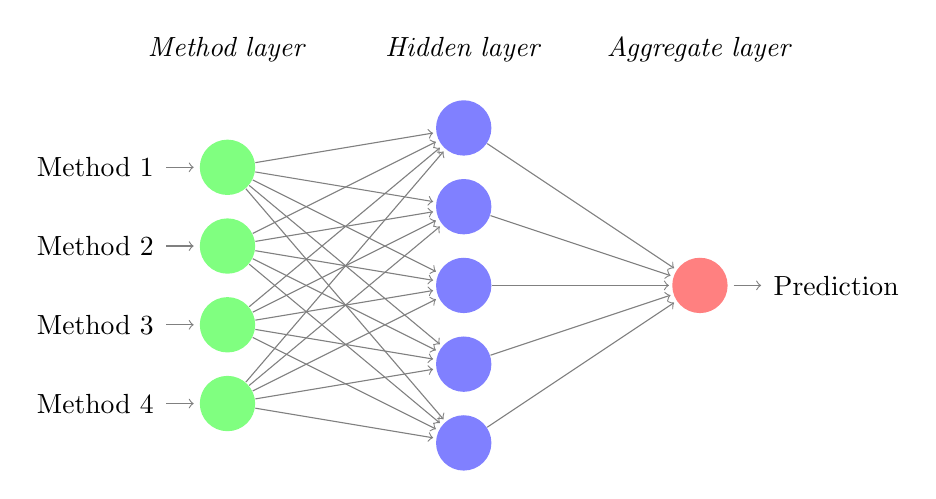
\begin{tikzpicture}[shorten >=1pt,->,draw=black!50, node distance=\layersep]

    \tikzstyle{every pin edge}=[<-,shorten <=2pt]
    \tikzstyle{neuron}=[circle,fill=black!25,minimum size=20pt,inner sep=0pt]
    \tikzstyle{input neuron}=[neuron, fill=green!50];
    \tikzstyle{output neuron}=[neuron, fill=red!50];
    \tikzstyle{hidden neuron}=[neuron, fill=blue!50];
    \tikzstyle{annot} = [text width=10em, text centered]

    % Draw the input layer nodes
    \foreach \name / \y in {1,...,4}
    % This is the same as writing \foreach \name / \y in {1/1,2/2,3/3,4/4}
        \node[input neuron, pin=left:Method \y] (I-\name) at (0,-\y) {};

    % Draw the hidden layer nodes
    \foreach \name / \y in {1,...,5}
        \path[yshift=0.5cm]
            node[hidden neuron] (H-\name) at (\layersep,-\y cm) {};

    % Draw the output layer node
    \node[output neuron,pin={[pin edge={->}]right:Prediction}, right of=H-3] (O) {};

    % Connect every node in the input layer with every node in the
    % hidden layer.
    \foreach \source in {1,...,4}
        \foreach \dest in {1,...,5}
            \path (I-\source) edge (H-\dest);

    % Connect every node in the hidden layer with the output layer
    \foreach \source in {1,...,5}
        \path (H-\source) edge (O);

    % Annotate the layers
    \node[annot,above of=H-1, node distance=1cm] (hl) {\emph{Hidden layer}};
    \node[annot,left of=hl] {\emph{Method layer}};
    \node[annot,right of=hl] {\emph{Aggregate layer}};
  \end{tikzpicture}

  \vspace{1em}
  \caption[User Meta Model Network]{
    The use of a multilayer perceptron for personalized model aggregation.
    This example takes the results from 4 different modeling methods,
    feeds them into a pretrained personalized neural net,
    and creates a combined prediction as output.}
  \label{fig:metanetwork}
\end{figure}


The prediction algorithm is given in Listing \ref{code:prediction}.

\begin{figure*}
  \lstinputlisting[
    label=code:prediction,
    caption={The algorithm that performs prediction,
    i.e. estimating the unknown rating from user $u$ to item $i$.}
  ]{../code/prediction}
\end{figure*}



\section{Prediction Aggregation}

Adaptive prediction aggregation means combining the results
from multiple scalar predictors conditioned on the current context.
As mentioned, we have two levels of predictors.
The first level is a set of traditional recommender systems
that produce estimations of unknown ratings between users and items.
The second level is another set of recommender systems 
that predict how accurate each of the first level recommenders will be.
There are two distinct phases when using adaptive recommenders:

\begin{enumerate*}
  \item The modeling phase creates the user models for both levels.
  \item The prediction phase uses the created models to estimate ratings.
\end{enumerate*}

We shall first explain the modeling phase, then the prediction phase.
The next section will explain a similar situation where
we wish to do \emph{adaptive rank aggregation} by 
combining ordered lists of results, depending on the current user and item.


\subsection{Modeling Phase}

Listing \ref{code:training} gives the basic algorithm for training
our models. The input to this method is the standard ratings matrix,
and a set of untrained modeling methods (in this case,
untrained recommender systems).

\begin{algorithm}
  \begin{algorithmic}[1]
  \REQUIRE ratings: The ratings matrix
  \REQUIRE methods: The set of modeling methods
  \ENSURE  rating\_models, error\_models: trained rating and error models 
    \STATE $rating\_models \gets \emptyset$
    \STATE $error\_models \gets \emptyset$
    \FORALL{$m \in methods$}
      \STATE $sample \gets \mathrm{BootstrapSample}(ratings)$
      \STATE $rating\_models_m \gets \mathrm{TrainModel}(m, sample)$
      \STATE $error\_models_m  \gets \mathrm{TrainErrorModel}(rating\_models_m, ratings)$
    \ENDFOR 
  \RETURN $(rating\_models, error\_models)$
  \end{algorithmic}
  \caption[Adaptive Prediction Aggregation Modeling]{Adaptive Prediction Aggregation Modeling
  }
  \label{code:training}
\end{algorithm}

An important question is how we should split the ratings data.
In this scenario, we need to split the data for a number of purposes.
The following sets must be created during training:

\begin{enumerate*}
  \item Training sets for the standard recommenders.
  \item Training sets for the error estimation models.
  \item A testing set to measure the performance of our final system.
\end{enumerate*}

Constructing these subsets of the available data is a common task in ensemble learning
\cite[p7]{Polikar2006}.
As seen in Listing \ref{code:training}, we use an approach called 
\emph{bootstrap aggregation}, also known as \emph{bagging}
(introduced by \cite{Breiman1996}).
Originally, bagging is used by ensemble learning classification methods, where multiple classifiers are 
trained by uniformly sampling a subset of the available training data. 
Each model is then trained on one of these subsets, and the models are aggregated by averaging their individual predictions.

Formally, given a training set $D$ with $n$ items, bagging creates $m$ new training sets of size $n' \leq n$ by sampling
items from $D$ uniformly and with replacement. 
In statistics, these types of samples are called \emph{bootstrap samples}.
If $n'$ is comparable in size to $n$, there will be some items
that are repeated in the new training sets.

Bagging suits our needs for a few reasons. First, it helps create disjoint predictors, 
since each predictor is only trained (or specialized for) a subset of the available data.
When using multiple similar recommenders, this means we can create specialized models
for parts of the data with a higher performance than if they were trained on the entire dataset.
Second, bagging allows us to easily train the underlying modeling methods without any complex partitioning of the data.
To partition and use the available data, we use the following algorithm:

\begin{enumerate*}
  \item Split the entire dataset into a training and testing set.
  \item Train modeling methods through bootstrap aggregation of the training set.
  \item Train error models from the complete training set.
  \item Test the resulting system with the initial testing set.
\end{enumerate*}

Each modeling method is trained in ways specific to their implementation. 
Model-based approaches create pre-built structures and provide offline training,
while heuristic methods simply store the data for future computation.
Either way, it is up to each modeling method what it does with the supplied training data.
The result of this algorithm is a set of trained rating models and error models.

\begin{algorithm}
  \begin{algorithmic}[1]
  \REQUIRE ratings: the ratings matrix
  \REQUIRE rating\_model: a recommender system user model
  \ENSURE error\_model: a trained error model for this method
    \STATE $errors \gets [[]]$
    \FORALL{$user,item,rating \in ratings$}
        \STATE $errors_{user,item} \gets | ratings_{user,item} - \mathrm{Predict}(rating\_model, user, item) |$
    \ENDFOR 
    \STATE $error\_method \gets \mathrm{NewModelingMethod}(SVD)$
    \STATE $error\_model  \gets \mathrm{TrainModel}(error\_method, errors)$
  \RETURN $error\_model$
  \end{algorithmic}
  \caption[Prediction Error Modeling]{Prediction Error Modeling}
  \label{code:trainerrormodel}
\end{algorithm}

Listing \ref{code:trainerrormodel} shows an algorithm for training the error models.
The input is the entire ratings matrix, and a trained recommender model
that this error model should represent.
We first create the aforementioned error matrix by estimating
predictions for each known combination in the ratings data.
The $\mathrm{NewModelingMethod}$ call simply creates a new, untrained
recommender model of some pre-specified $type$
(in this case, a new SVD-based model, but any applicable RS will do).
A new model is then trained based on the created error matrix,
and returned as our new $error\_model$.

When the computations of the algorithm in Listing \ref{code:training} is complete,
we have a set of trained recommender systems, and a set of trained error models.
Each recommender model has a corresponding error model,
forming two layers, that we shall use when performing predictions.


\subsection{Prediction Phase}

In the prediction phase of adaptive prediction aggregation,
we wish to use our layers of trained models to produce adaptive
combinations of multiple predictions and accuracy estimations.
Listing \ref{code:prediction} gives the basic algorithm.

\begin{algorithm}
  \begin{algorithmic}[1]
  \REQUIRE user, item: a user and an item
  \REQUIRE rating\_models: the set of trained modeling methods 
  \REQUIRE error\_models: the set of trained error models
  \ENSURE  prediction: the predicted relevance of the item to the user
    \STATE $ratings \gets \emptyset$
    \STATE $errors  \gets \emptyset$
    \FORALL{$m \in rating\_models$}
      \STATE $ratings_{m} \gets \mathrm{Predict}(rating\_models_m, user, item)$
      \STATE $errors_{m}  \gets \mathrm{Predict}(error\_models_m, user, item)$
    \ENDFOR 
    \STATE $errors \gets \mathrm{Normalize}(errors)$
    \STATE $prediction \gets 0$
    \FORALL{$m \in rating\_models$}
      \STATE $weight_m \gets 1 - error_m$
      \STATE $prediction \gets prediction + weight_m \times ratings_m$
    \ENDFOR
 
  \RETURN $prediction$
  \end{algorithmic}
  \caption[Adaptive Prediction Aggregation]{Adaptive Prediction Aggregation
  }
  \label{code:prediction}
\end{algorithm}

The first input is the user and item for which we wish to predict a rating.
We assume that this rating is unknown --- predicting ratings for known combinations
would mean recommending items the user has already seen and considered
(however, if we are dealing with a task such as personalized search,
these known ratings are important, as we shall see in the next section).

The other inputs are the trained rating models, and the corresponding error models.
The algorithm begins by creating empty sets for predicted ratings and errors.
Next, each modeling method is used to predict ratings, and their error models to predict errors.
Note that each step in the first for-loop is independent of each other, and both steps
inside the for loop are also independent. 
This is then an algorithm well suited for parallelization.
In a MapReduce framework, this for loop would be run as a $\mathrm{map}$ operation,
where the input user and item is mapped over the sets of modeling methods
(see Appendix \ref{appendix:implementation} for implementation details).

After the predictions have been collected, the errors are normalized,
i.e. converted to the range $[0,1]$, so that they sum to $1$.
This is vital before last stage of the prediction algorithm,
which weighs each prediction from the different rating models.
The last step corresponds to the previously explained $\mathrm{reduce}$ operation,
that combines multiple scores into one final result.
The weight of each method is computed as $1 - error$, where $error$ 
is the normalized error for this method, for the current user and item.
Each rating prediction is then weighted, and combined to form the final,
adaptively aggregated prediction.

There is an important performance different between the modeling and prediction phases:
While the modeling phase is the most computationally expensive,
it can be performed independently of making predictions.
As the prediction phase is when the user has to wait for the system,
this is where performance is most important.
Naturally, as users rate more items and new items arrive,
the models have to be recreated based on this new reality.
However, as the modeling phase is an offline operation,
the training can be performed in the background, while new
and computatinally efficient predictions are always available.




\section{Rank Aggregation}
\label{sec:methods:rank}

It is time to see how to do \emph{adaptive rank aggregation}. 
Rank aggregation means combining sorted lists of items.
In this scenario, each modeling method takes the current user as input, and produces a
list of items ranked in order of rating (see also Section \ref{sec:theory:rank}).

Aggregating lists is desirable in a number of situations.
Often we wish to produce lists of recommended items, not just estimate the rating of a single user/item pair.
Consider the task of personalizing a list of search results
(see Section \ref{sec:search}). The important part is not the score
given to each result, but rather the order in which they appear.
The underlying technology stays the same. A number of recommenders are used to predict the ratings
of items to users. However, to do rank aggregation, another layer is added, that requests lists from each method,
not only singular items.

Because it is such an important use case, we shall use personalized search to present our approach to adaptive rank aggregation.
In addition to the standard recommenders, we have an information retrieval method,
as introduced in Section \ref{sec:ir}.
The IR method takes in a user-initiated query (a collection of words or a sentence), and returns a number of 
search results, in an ordered list.
In traditional personalized search, a recommender system can then be used to estimate a rating for each of the returned items,
and re-sort, or re-score, the results list (e.g. \citet[p3]{Xu2008}).

The key insight is that both the IR method and the recommender systems form \emph{input signals}
(see Section \ref{subsec:signals}).
An input signal is some measure of how each item should be ranked in the final results list.
The relevance scores returned from our IR ranking functions are signals,
and the predicted ratings from each recommender systems are signals.
Adaptive aggregation then entails estimating \emph{how accurate each of these signals are likely to be for the current user and item}.
This is almost the same task as in adaptive prediction aggregation, only in a list-oriented fashion.

There is an important difference. 
The IR methods should be used to constrict the range of items worked on by the recommender systems.
As the IR methods identify items that may be relevant to the users query, these are the items we wish the recommender systems to work on.
This goes back to the previously mentioned difference between \emph{search} and \emph{recommendations}:

\begin{itemize*}
  \item Recommenders find relevant items the user does not already know exists.
  \item Search engines find relevant items the user knows or hopes exists.
\end{itemize*}

The difference lies in the knowledge of existence.
As personalized search is still a search task, the IR methods should determine the set of items that might be relevant.
Their relevance scores for these items becomes the first input signals.
The recommender systems works on this set of items, re-scoring each as needed.
We still have the adaptive layer that estimates how well each signal will perform for the current user and item.
This is especially important considering that we may have multiple IR methods that define multiple sets of relevant items.
The final result is an adaptive combination of the rating and accuracy predictions for each signal,
as seen in Figure \ref{fig:adaptiverank}.
Let us now see how the modeling and prediction phases are performed in adaptive rank aggregation.

\begin{figure}[t]
  \center
  \def\layersep{3cm}
  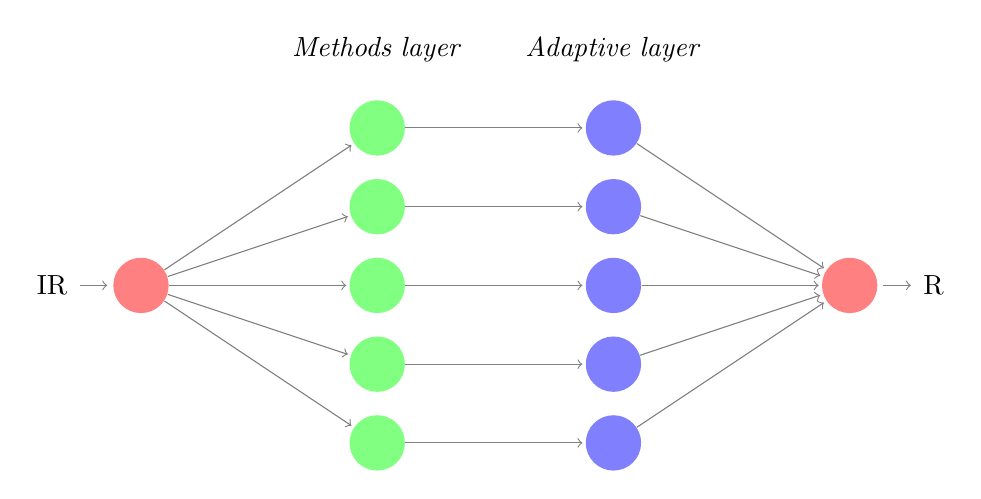
\begin{tikzpicture}[shorten >=1pt,->,draw=black!50, node distance=\layersep]

    \tikzstyle{every pin edge}=[<-,shorten <=2pt]
    \tikzstyle{neuron}=[circle,fill=black!25,minimum size=20pt,inner sep=0pt]
    \tikzstyle{input neuron}=[neuron, fill=green!50];
    \tikzstyle{output neuron}=[neuron, fill=red!50];
    \tikzstyle{hidden neuron}=[neuron, fill=blue!50];
    \tikzstyle{annot} = [text width=10em, text centered]
    
    \node[output neuron, pin=left:IR] (IR) at (0,-3) {};
    
    \node[input neuron] (M-1) at (\layersep, -1) {};
    \node[input neuron] (M-2) at (\layersep, -2) {};
    \node[input neuron] (M-3) at (\layersep, -3) {};
    \node[input neuron] (M-4) at (\layersep, -4) {};
    \node[input neuron] (M-5) at (\layersep, -5) {};
    
    \node[hidden neuron] (E-1) at (\layersep*2, -1) {};
    \node[hidden neuron] (E-2) at (\layersep*2, -2) {};
    \node[hidden neuron] (E-3) at (\layersep*2, -3) {};
    \node[hidden neuron] (E-4) at (\layersep*2, -4) {};
    \node[hidden neuron] (E-5) at (\layersep*2, -5) {};
    
    \node[output neuron,pin={[pin edge={->}]right:R}, right of=E-3] (O) {};
    
    \foreach \source in {1,...,5}
         \path (M-\source) edge (E-\source);
     
    \foreach \source in {1,...,5}
         \path (IR) edge (M-\source);
 
    \foreach \source in {1,...,5}
         \path (E-\source) edge (O);
    
    \node[annot, above of=M-1, node distance=1cm] (hl) {\emph{Methods layer}};
    \node[annot, right of=hl] {\emph{Adaptive layer}};

  \end{tikzpicture}

  \vspace{1em}
  \caption[Stacked Rank Aggregation]{
    Stacked Rank Aggregation: 
    An IR method returns a results list of possibly related items, each with a ranking score.
    The methods layer estimates ratings for each item in the results list.
    The adaptive layer predicts how accurate ach of these ratings are likely to be.
    Finally, the ranking scores, ratings and accuracy estimations are combined
    into one result list, R.
  }
  \label{fig:adaptiverank}
\end{figure}


\subsection{Modeling Phase}

We shall only deal with settings where we have a single IR method.
While multiple IR methods and corresponding error models is an interesting
setting, we are most interested in using the IR method for constraining the Item-space considered by the recommender systems.
As we shall see, this does not introduce many changes to our algorithms.

The modeling phase for the recommender system stays the same, with one important change.
As we are dealing with a search engine, we might not have an explicit ratings matrix to rely on.
Most feedback we can gather from user initiated searches are from query logs.
These logs show the current user, query, and the item that is finally selected after the query is performed.
Query log mining is a common approach in personalized search
(e.g. \cite{Liu2002, Sugiyama2004, Shen2005, Speretta2000}).
By mining query logs we can create an implicit ratings matrix.
Each populated cell represents a selected item.

For example, \cite{Venetis2011} shows an interesting approach where they use requests for directions
from online map services to infer implicit ratings:
when a user asks for the directions from A to B, this is taken 
as a vote from this user that location B is interesting.
This is just one of many ways implicit ratings matrices can be mined.

The values in this implicit ratings matrix can take many forms.
If we only care about selected items, binary ratings may suffice:
selected items are then represented by a $1$ in the ratings matrix.
These ratings can be further improved by considering different metrics, including:

\begin{itemize*}
  \item Time spent before selecting the item.
  \item The items initial placement and the effort required to identify it.
  \item How far the user was willing to scroll before clicking the item.
  \item Whether or not the user resubmitted the same query shortly after.
\end{itemize*}

Based on these and other similar metrics, one can achieve quite accurate implicit ratings.
Naturally, ratings can also be gathered from other sources.
If we have more data on each user, or know of secondary systems such as social networks
or other systems where ratings are present, these can be used to augment the implicit ratings matrix
(e.g. \cite{Carmel2009}).
There are also search systems where we already have explicit ratings.
Consider, for instance, the use case of searching for movies on a movie rating site,
or searching for people in a social network.
In these cases, we have explicit ratings that can be used to train the recommender models.

A thorough explanation of turning query logs into ratings matrices
is beyond the scope of this thesis. Extensive research already
looks at how implicit user model information may be gleaned
from simple query logs. Examples include \cite{Joachims2007},
\cite{Lee2005}, \cite{Agichtein2006}, \cite{Mobasher} and
\cite{Speretta2000}.

As in prediction aggregation, the strength of our resulting system is in large part dependent on the accuracy of our ratings.
This means that deciding and understanding how implicit ratings are created, or 
finding auxiliary sources to provide explicit ratings, is a critical step.
The algorithms are only as strong as the data they use.
Methods for personalized search may work best in settings where we have explicit ratings,
or can gather explicit ratings from secondary sources, for example from external social networks or publishing platforms.

When we have the implicit or explicit ratings matrix, the modeling phase
consists of two parts. Training the IR models and the recommender models.
The recommender models are trained as before, given in Listing \ref{code:training}.
The one or more IR methods are not trained with a ratings matrix,
but with the items and their respective data.
Of course, the actual IR modeling method depends on the IR system itself.
However, as a through explanation of IR systems is outside our scope,
we assume that the IR model is trained with the system's items,
and that it returns relevant items when given a query.


\clearpage
\subsection{Prediction Phase}

\begin{algorithm}[t]
  \begin{algorithmic}[1]
  \REQUIRE user: the current user
  \REQUIRE items: the set of all items and their meta-data
  \REQUIRE query: the user initiated query
  \REQUIRE ir\_model: a trained IR model
  \REQUIRE rating\_models: the set of trained modeling methods 
  \REQUIRE error\_models: the set of trained error models
  \ENSURE  results: the adaptively sorted list of results
    \STATE $ratings \gets \emptyset$
    \STATE $errors  \gets \emptyset$
    \STATE $results \gets \mathrm{Search}(ir\_model, items, query)$
    
    \FORALL{$item \in results$}
      \FORALL{$m \in rating\_models$}
        \STATE $ratings_{m,item} \gets \mathrm{Predict}(rating\_models_m, user, item)$
        \STATE $errors_{m,item}  \gets \mathrm{Predict}(error\_models_m, user, item)$
      \ENDFOR 
    \ENDFOR
    \STATE $errors \gets \mathrm{Normalize}(errors)$

    \FORALL{$item, ir\_score \in results$}
      \STATE $prediction \gets w_{IR} \times ir\_score$
      \FORALL{$m \in rating\_models$}
        \STATE $weight_{item} \gets 1 - error_{m,item}$
        \STATE $prediction \gets prediction + weight_m \times ratings_{m,item}$
      \ENDFOR
      \STATE $item_{prediction} \gets prediction$
    \ENDFOR
    
    \STATE $results \gets \mathrm{SortByPredictions}(results)$
  \RETURN $results$

  \end{algorithmic}
  \caption[Adaptive Rank Aggregation]{Adaptive Rank Aggregation}
  \label{code:rank:prediction}
\end{algorithm}

The prediction phase is where adaptive rank aggregation differs most from adaptive prediction aggregation.
Listing \ref{code:rank:prediction} gives the basic algorithm.
As input, instead of one item, we have the entire set of items, and a query.
We run the query and items through the IR model to get the constrained set of items ($results$).
Each of the recommender methods is then run for each of the items in the results list.
As before, the first for-loop can be performed in parallel.
Each call to $Predict$ is independent of the other operations,
allowing us to perform it as a $map$ operation.

As before, the error estimations are normalized before converting them to weights.
Since we are dealing with two dimensions of errors, for each item and each method,
the errors are normalized across items.
For each item, the errors from the recommenders fall in the range $[0,1]$ and sum to $1$.

After each item in the results list has an IR score, a set of predictions, and a corresponding set of 
error predictions, the adaptive aggregated prediction is computed. 
Because we do not care of the final score we set the initial predictions to be the IR scores.
The recommender systems simply add or subtract from this initial score.
This means that the resulting predictions will not be in the same range as the known ratings,
but since we are only interested in the order of the items, not the actual rating, this is not a problem.

An important coefficient is the $w_{IR}$ (IR weight),
which determines how much the IR method should decide of the final ranking.
This is first and foremost adjusted to ensure that the IR scores
are on a similar scale as the predicted ratings.
At the same time, this weight determines how 
much the IR score influences the final placement of an item in the results list.
In the next chapter, we shall see how the choice this parameter 
influences the ranked results lists.

After computing the predictions for each item in the results list, 
we sort the list by the item predictions, and return the list.
The resulting list is adaptively sorted based on the current user and the specific items in the list,
achieving adaptive rank aggregation.

Listing \ref{code:rank:prediction} considers rank aggregation in a scenario with a single IR model.
In the case of more IR models,
we would combine the scores for each item returned by the different models.
In this case, estimating the accuracy of each IR model in the same way as the recommender systems
would provide another level of personalization.
Just as each RS works differently for each element, each IR model
may have varying applicabiltiy to each item.
At the same time, each user might place a different importance on each IR model.

This would be a simple extension of our prediction algorithm.
The most important question becomes how to estimate the error matrix for an IR model.
There are many ways to do this.
For example, the error for each query could be based on how 
how often the element in question is selected for the current query.
Another error might be based on the difference between
the optimal placement (based on click-through rates)
and the actual placement of an item in the result list.

However, as this is outside the scope of this thesis, 
we shall stick to situations where we have a single IR model.
Experiment 3 in the next chapter will show how this IR model can be used in different ways
by varying the IR weight.





\hr

In this chapter, we have seen how to perform stacked user modeling.
It is now time to see how this model performs.
The next chapter will test the viability of 
our model and answer our three hypotheses.

